%% Languages: norsk				
%%						english			
%% Styles:		twoside, 		The margins will differ dependent on right/left pages
%%						openright		The first page is a "right" page
%%  indexes:		listings		Show figure list, table list
%%						glossary		Show glossary and abbreviation list
%%						todo				Show list of todo-notes in documents
%%						%
\documentclass[english]{gucreport}
\projdate{ \today }
\projvers{ 1.0 }

\courseid{ IMT3521 }
\coursename{  Security Planning and Incident Management }
\projteacher{ Marie Elisabeth Gaup Moe }

\appnumber{ N/A } %	number of appendixes
								%	currently auto calculated but might be wrong
\pagecount{ \pageref{LastPage} }

\projtitle{ Smoking Games }
\projsubtitle{ Contingency Plan }

\projauthor{ Adrián Alberdi Ainziburu }
\projauthorid{ 130197 }
\projauthorA{ Leonard Eschenbaum }
\projauthorAid{ 131721 }
\projauthorB{ }
\projauthorBid{ }
\projauthorC{ }
\projauthorCid{ }
\projauthorD{ }
\projauthorDid{ }

%\renewcommand{\familydefault}{\sfdefault}
%\rmfamily

\begin{document}
	%%%
%%	Dictonary
%%		\newglossaryentry{unique_id}{name={Term}, description={Description}}
%%
%\newglossaryentry{}{name={}, description={}}
\newglossaryentry{lorem}{name={Lorem ipsum}, description={AKSJDKLAJSLKD 12"/(/}}

%%
%%	Abbreviations
%%		\nomenclature{Abbreviation}{Description}
%%
%\nomenclature{}{}
\nomenclature{OS}{Operating System}
\nomenclature{LTS}{Long Term Support}
\nomenclature{ROTFWLMAO}{Rolling On The Floor While Laughing My Ass Off}


	\makefrontpages
	\tableofcontents
	\showindex		%%lists of figures, codes, tables, glossary, etc
	
	%% Chapters for the text
	\section{Business Description}
Smoking Games is a video game development and digital distribution company founded in 2008 by a group of 5 international students from Gj\o vik University College. The company is located in Tenerife, Spain.
\section{Business Overview}
Smoking Games started as a small video game developer company. At the beginning they distributed their games through other distributers. After the great hit of a video game called ''full life'', they decided to start distributing their games on their own.\\
In 2010, after 2 years in the development business, Smoking Games became a video game developer and digital distributor enterprise. At the start they only distributed their own games. With the growth of the enterprise Smoking Games got many offers from other game developers to distribute their games. Like this Smoking Games decided that they will distribute also other developers creation in their digital distribution section. At this point the distribution software was named Smoke. \\
2011 was a great year for Smoking Games, the growth of computer gaming in this year helped consolidating the enterprise and Smoke became the gaming platform for everyone. In Smoking Games they didn't think it was enough, as their mission states: "Always creating and innovating". So they took the next step, a cloud service for saving games and cross platform gaming. Playing on two devices always moving forward in a shared game. In the other hand ''full life 3'' was released during this year getting Smoking Games a very good position in the market as a trusted game developer.\\
In 2012, after 4 years in a rented placement the head quarter of Smoking Games moved to a newly owned location. Taking advantage of this growth the whole enterprise grew. It redefined in this year still at the same size of 35 employees fixed plus some external services. Even though the enterprise organization is quite horizontal, the shares and benefits belong to the employees and bosses in the same amount, they keep a minimun organization for political purposes. The hierarchy of the enterprise is the one shown in figure \ref{fig:org_hierarchy}.

\begin{figure}[htpb]\centering
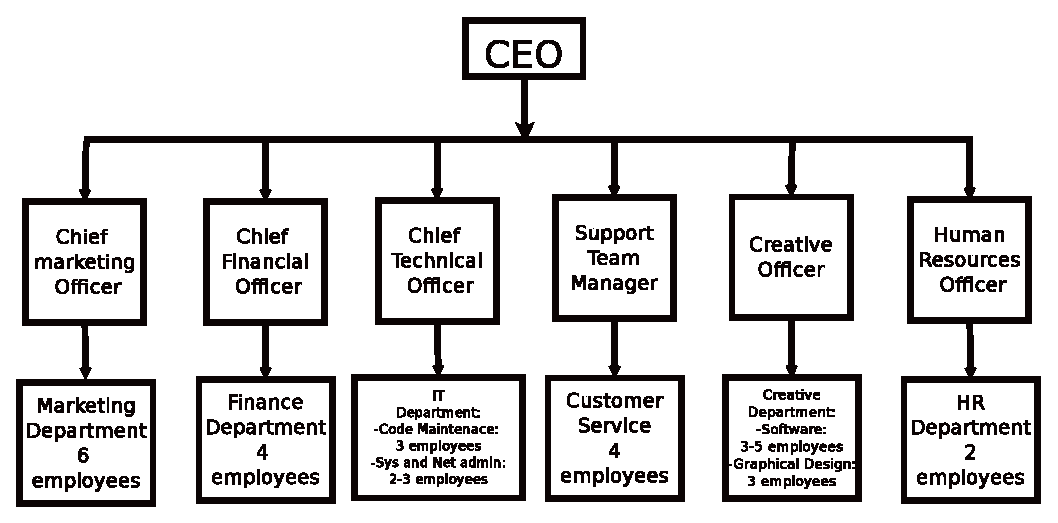
\includegraphics[ width={0.7\textwidth} ] {pictures/Organizational_hierarchy}
\caption{Organizational hierarchy}
\label{fig:org_hierarchy}
\end{figure}
\newpage
\noindent The main source of income for Smoking Games is by selling their own games, those games give a 100\% of the price back. The games produced by other companies are a different story: for every game and developer Smoking Games makes a different contract, going from the 75 to the 50\%money of the solds in the distribution price.\\
Smoking Games is located in a building in Tenerife, Spain. The building next to it is one of the main hubs for telefonica SA, main internet company in Spain. Like this the internet conection is much more ensured. This is important because most of the business of Smoking Games are done over the internet.

\section{Assets}
Smoking Games' assets can be categorized into tangible and intangible assets. Every service consulted or used by Smoking Games which benefits them or is more or less essential for business processes is considered an asset.
\subsection{Tangible Assets}
Besides the obvious assets like building, computers or other hardware, power, water and data and telecommunication services are essential for Smoking Games' business processes and procedures and are therefore considered an asset because when one of these services is not available anymore it will inflict damage on their business economy. All tangible assets are shown in table \ref{tab:TangibleAssets}.
\begin{table}[h]
	\centering
	\begin{tabular}{l | l}
		\textbf{Asset} & \textbf{Economic Benefit}\\\hline\hline
		\parbox[t]{6cm}{Office Building and Offices} & \parbox[t]{6cm}{Provides space for employees}\\\hline
		\parbox[t]{6cm}{Office Equipment} & \parbox[t]{6cm}{Provides the necessary equipment for employees}\\\hline
		\parbox[t]{6cm}{in-house IT-system \& File Storage} & \parbox[t]{6cm}{Provides maintainability and storage of customer information and applications}\\\hline
		\parbox[t]{6cm}{Server Farm} & \parbox[t]{6cm}{Provides accessibility for customers and employees}\\\hline
		\parbox[t]{6cm}{Other Machines} & \parbox[t]{6cm}{Used for the production of goods}\\\hline
		\parbox[t]{6cm}{Other Hardware} & \parbox[t]{6cm}{Used for different business processes}\\\hline
		\parbox[t]{6cm}{Access Control} & \parbox[t]{6cm}{Provides selective restriction of access to resources}\\\hline
		\parbox[t]{6cm}{External Security Services (e.g. security guard, alarm system, CCTV cameras)} & \parbox[t]{6cm}{Provides protection of other assets or people}\\\hline
		\parbox[t]{6cm}{Emergency Generator} & \parbox[t]{6cm}{Provides backup power}\\\hline
		\parbox[t]{6cm}{Data and Telecommunication, Power \& Water Services} & \parbox[t]{6cm}{Provides essential accessibility for business processes}\\\hline
		\parbox[t]{6cm}{Renovation} & \parbox[t]{6cm}{Provides maintainability of e.g. buildings}\\
	\end{tabular}
	\caption{Tangible Assets}\label{tab:TangibleAssets}
\end{table}
\subsection{Intangible Assets}
Smoking Games has been in the video game development business for six years and they have (as mentioned earlier) become well-known for its critically acclaimed games which helped them establish a business reputation in the public domain as well as their name is being recognized by people more and more often. Both have increased even more after they launched their distribution platform.\\
With the development of new software Smoking Games acquired new patents, logos, formulas and of course copyrights.\\
For additional assets see table \ref{tab:OtherTangibleAssets}. 
\begin{table}[h]
	\centering
	\begin{tabular}{l | l}
		\textbf{Asset Category} & \textbf{Asset}\\\hline\hline
		Information & \parbox[t]{7cm}{database information, employee contracts, consulting contracts, documentation,
manuals, procedures, incident response plans, business continuity plans, client data and
information, personal information, employee records, finance records, software licenses
and other}\\\hline
		Employees & \parbox[t]{7cm}{experience, information and knowledge}
	\end{tabular}
	\caption{Other Intengible Assets}\label{tab:OtherTangibleAssets}
\end{table}
\subsection{Asset Classification}
Smoking Games' assets can be classified as one of the following, with respect to their security needs.\\
\medskip
\begin{itemize}
	\item \textbf{Public:} Information and assets which is/are legally distributed/available and otherwise non-threatening to the company or its customers. This is for example information distributed through Smoking Games' website and information used in PR-campaigns.
	\item \textbf{Internal:} This is information and assets which is/are not a critical threat to the business, but is not meant to be available for the public. Disclosure of this information will yield minimal impact on the company’s daily operations, but will result in a breach of trust either with the public or customers. This involves work schedules, superficial business information and other.
	\item \textbf{Confidential:} Information and assets which is/are sensitive, business critical or otherwise legally obliged to be held confidential. Disclosure of this information will have an impact to the company in a way which disrupts or or threatens the company’s daily operations. This involves, among else, information related to the privacy act, business procedures, and client information.
\end{itemize}
\section{Business Procedures and Processes}

%%\subsection{Risk management process}



\subsection{Internal procedures}
The main internal procedure is the game creation. Besides this, as any other enterprise there are different internal procedures, human resources and IT maintenance, for example. The game creation follows the procedure shown in the figure \ref{fig:proc_game_creation} and is the following:

\begin{figure}[h] \centering
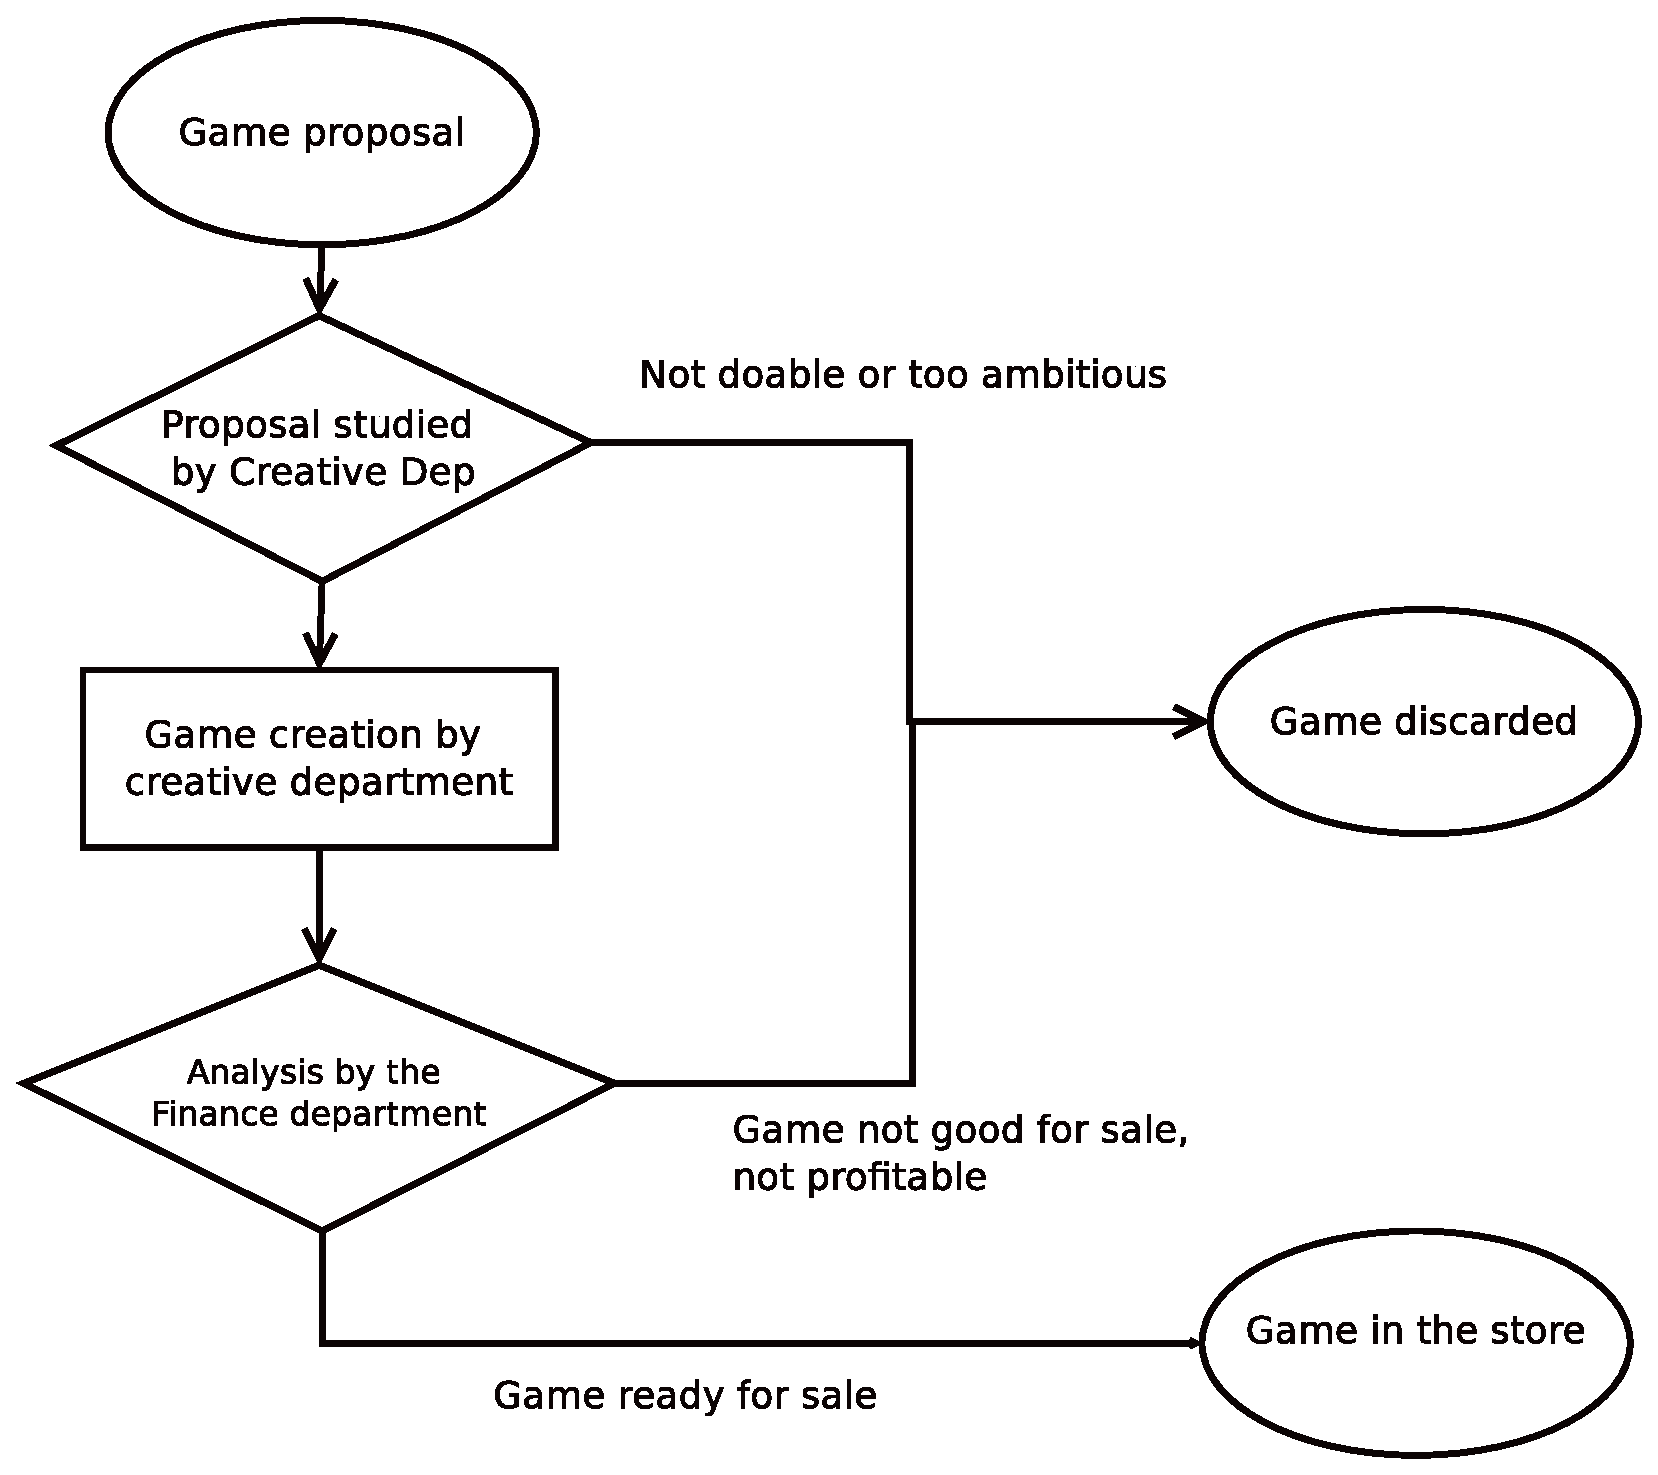
\includegraphics[width={0.7\textwidth}]{pictures/game_creation_process.eps}
\caption{Game creation process}
\label{fig:proc_game_creation}
\end{figure}

\begin {description}
\item{Idea creation: }This is the longer stage. It is a constant work in progress, during any stage the new ideas are taken in account. Once one project is finished a new idea is taken from the database.
\item{Idea study: }At this stage the idea is studied to check if it is doable, profitable and innovative. If it doesn't give the expected results the game idea is discarded.
\item{Game creation: }In this state the creative department starts the development of the project on itself. The development starts by programing the basic physics, story and the base program in general. When the 30\% of the estimated program is coded the design team starts working. At this early stage all the design is prepared for advertisement. While the game develops and the first alphas are launched the designers work more in the general graphics of the game.
\item{Game analysis: }When the game is around the 60\% through the development it's examined by the marketing department. If it gives clues for good and profitable sales it's approved and a marketing campaign is launched. If the game doesn't look good 	enough it's discarded.
\end {description}

\subsection{External procedures}
The main external procedure of Smoking games is the negotiation and signature of contracts with third party developers.

\begin{figure}[h]\centering
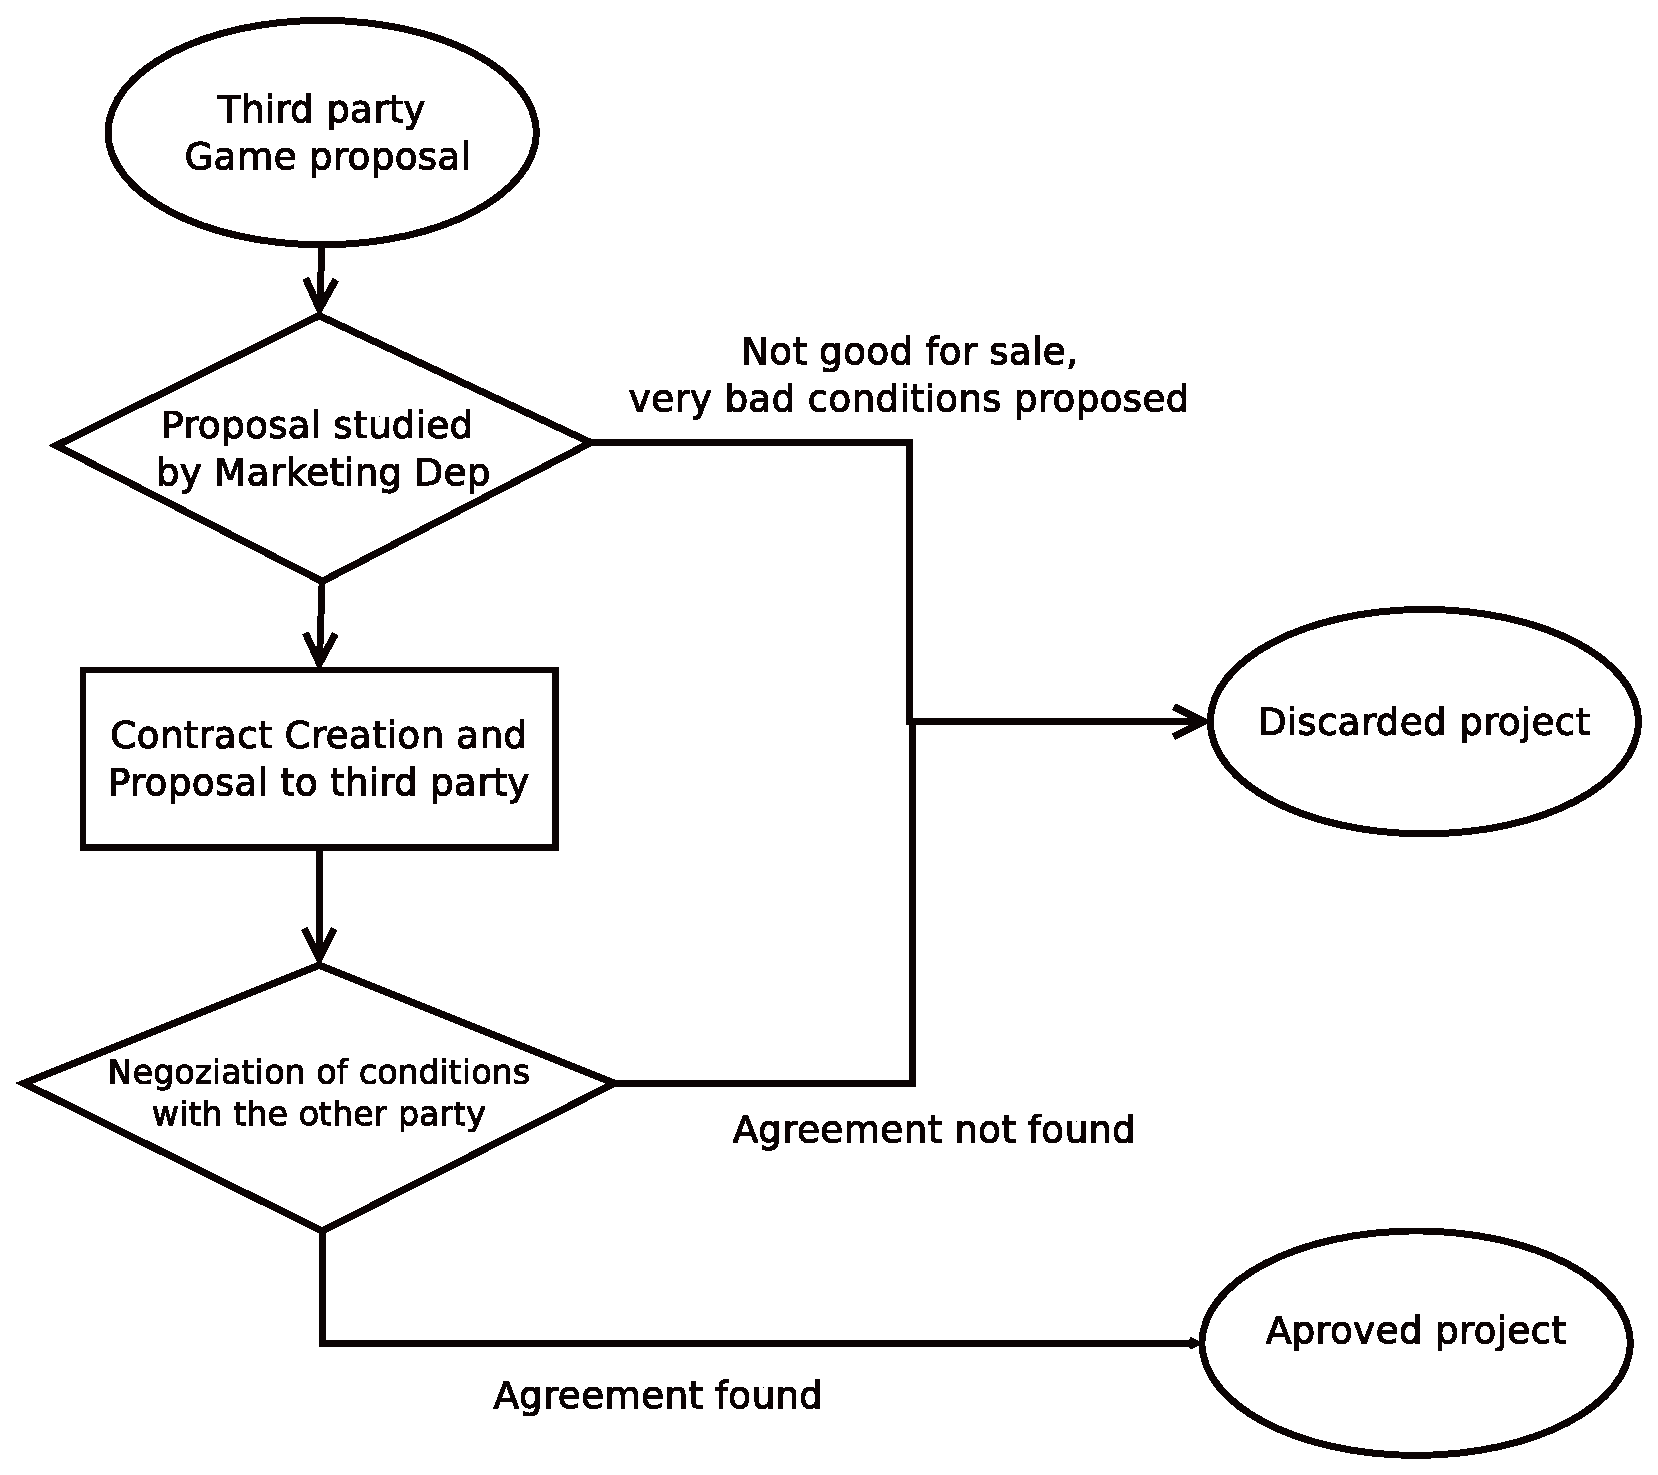
\includegraphics[ width={0.7\textwidth}]{pictures/third_party_game_process.eps}
\caption{Process for third party game distribution approval}
\label{fig:proc_third_party}
\end{figure}

This process as shown on the figure \ref{fig:proc_third_party} the process for signing a new contract is:

\begin{description}
\item{Project proposal reception: }The new game project is received in Smoking Games HQ.
\item{Project proposal analysis: }The project is given to the marketing department for market acceptance analysis and profit analysis. The marketing department will see the profitability of the project. In case the project doesn't give back a minimum the project will be discarded, and the developer told.
\item{Contract creation: }at this step the finance department will create a contract to present to the developer. The initial conditions of this contract have to have some flexibility for being able to negotiate. 
\item{Negotiation: }This newly created contract is presented and negotiated with the game developer. Depending on the result of this negotiation the project will be discarded or signed and validated.
\end{description}



An also important external procedure is the games sale through Smoke. This procedure is done using different payment options, credit card, pay pal or amazon payments, for example.
\newpage
\section{Network and Security}
To provide their customers security regarding their information, Smoking Games maintain their own in-house IT-system and file storage. This also gives the employees easy access to customer information with respect to the C.I.A. principles (confidentiality, integrity, availability).
\subsection{Network}
Smoking Games host their own Web services. Maintenance of these services and the rest of the network is the responsibility of Smoking Games' own IT department.\\
The company network is divided in, roughly speaking, three parts: the public network (DMZ), the internal network and the wireless network. An overview of the network topology is shown in figure \ref{fig:net_top}.\\
All connections between the outside and the internal network or the DMZ are being filtered by the external router which has a firewall included. The DMZ (demilitarized zone) contains public services such as a Web server or a VPN server (used for e.g. consulting purposes). Access to these services is restricted and handled by, as mentioned, the external router, which is configured to route packets between the outside and the DMZ differently than between the outside and the internal network. Additionally and IDS/IPS (incident detection/incident prevention system) is placed between the public network and the external router.\\
In case of a compromised external router all connectios between the outside and the internal network are being protected by an IDS/IPS and an internal router, which has additional filer lists implemented.\\
All information and data about customers or other business aspects are stored on the database server and file storage, respectively. Access to this data is handled by a router with a strictly configured firewall, so to avoid unauthorized access.\\
The rest of the internal network consists of work machines and a print server and printer.\\
A wireless network is also being provided, but it is not connected to the other network to avoid that information about customers or business projects is being stored on personal mobile devices.
\begin{figure}[h]\centering
	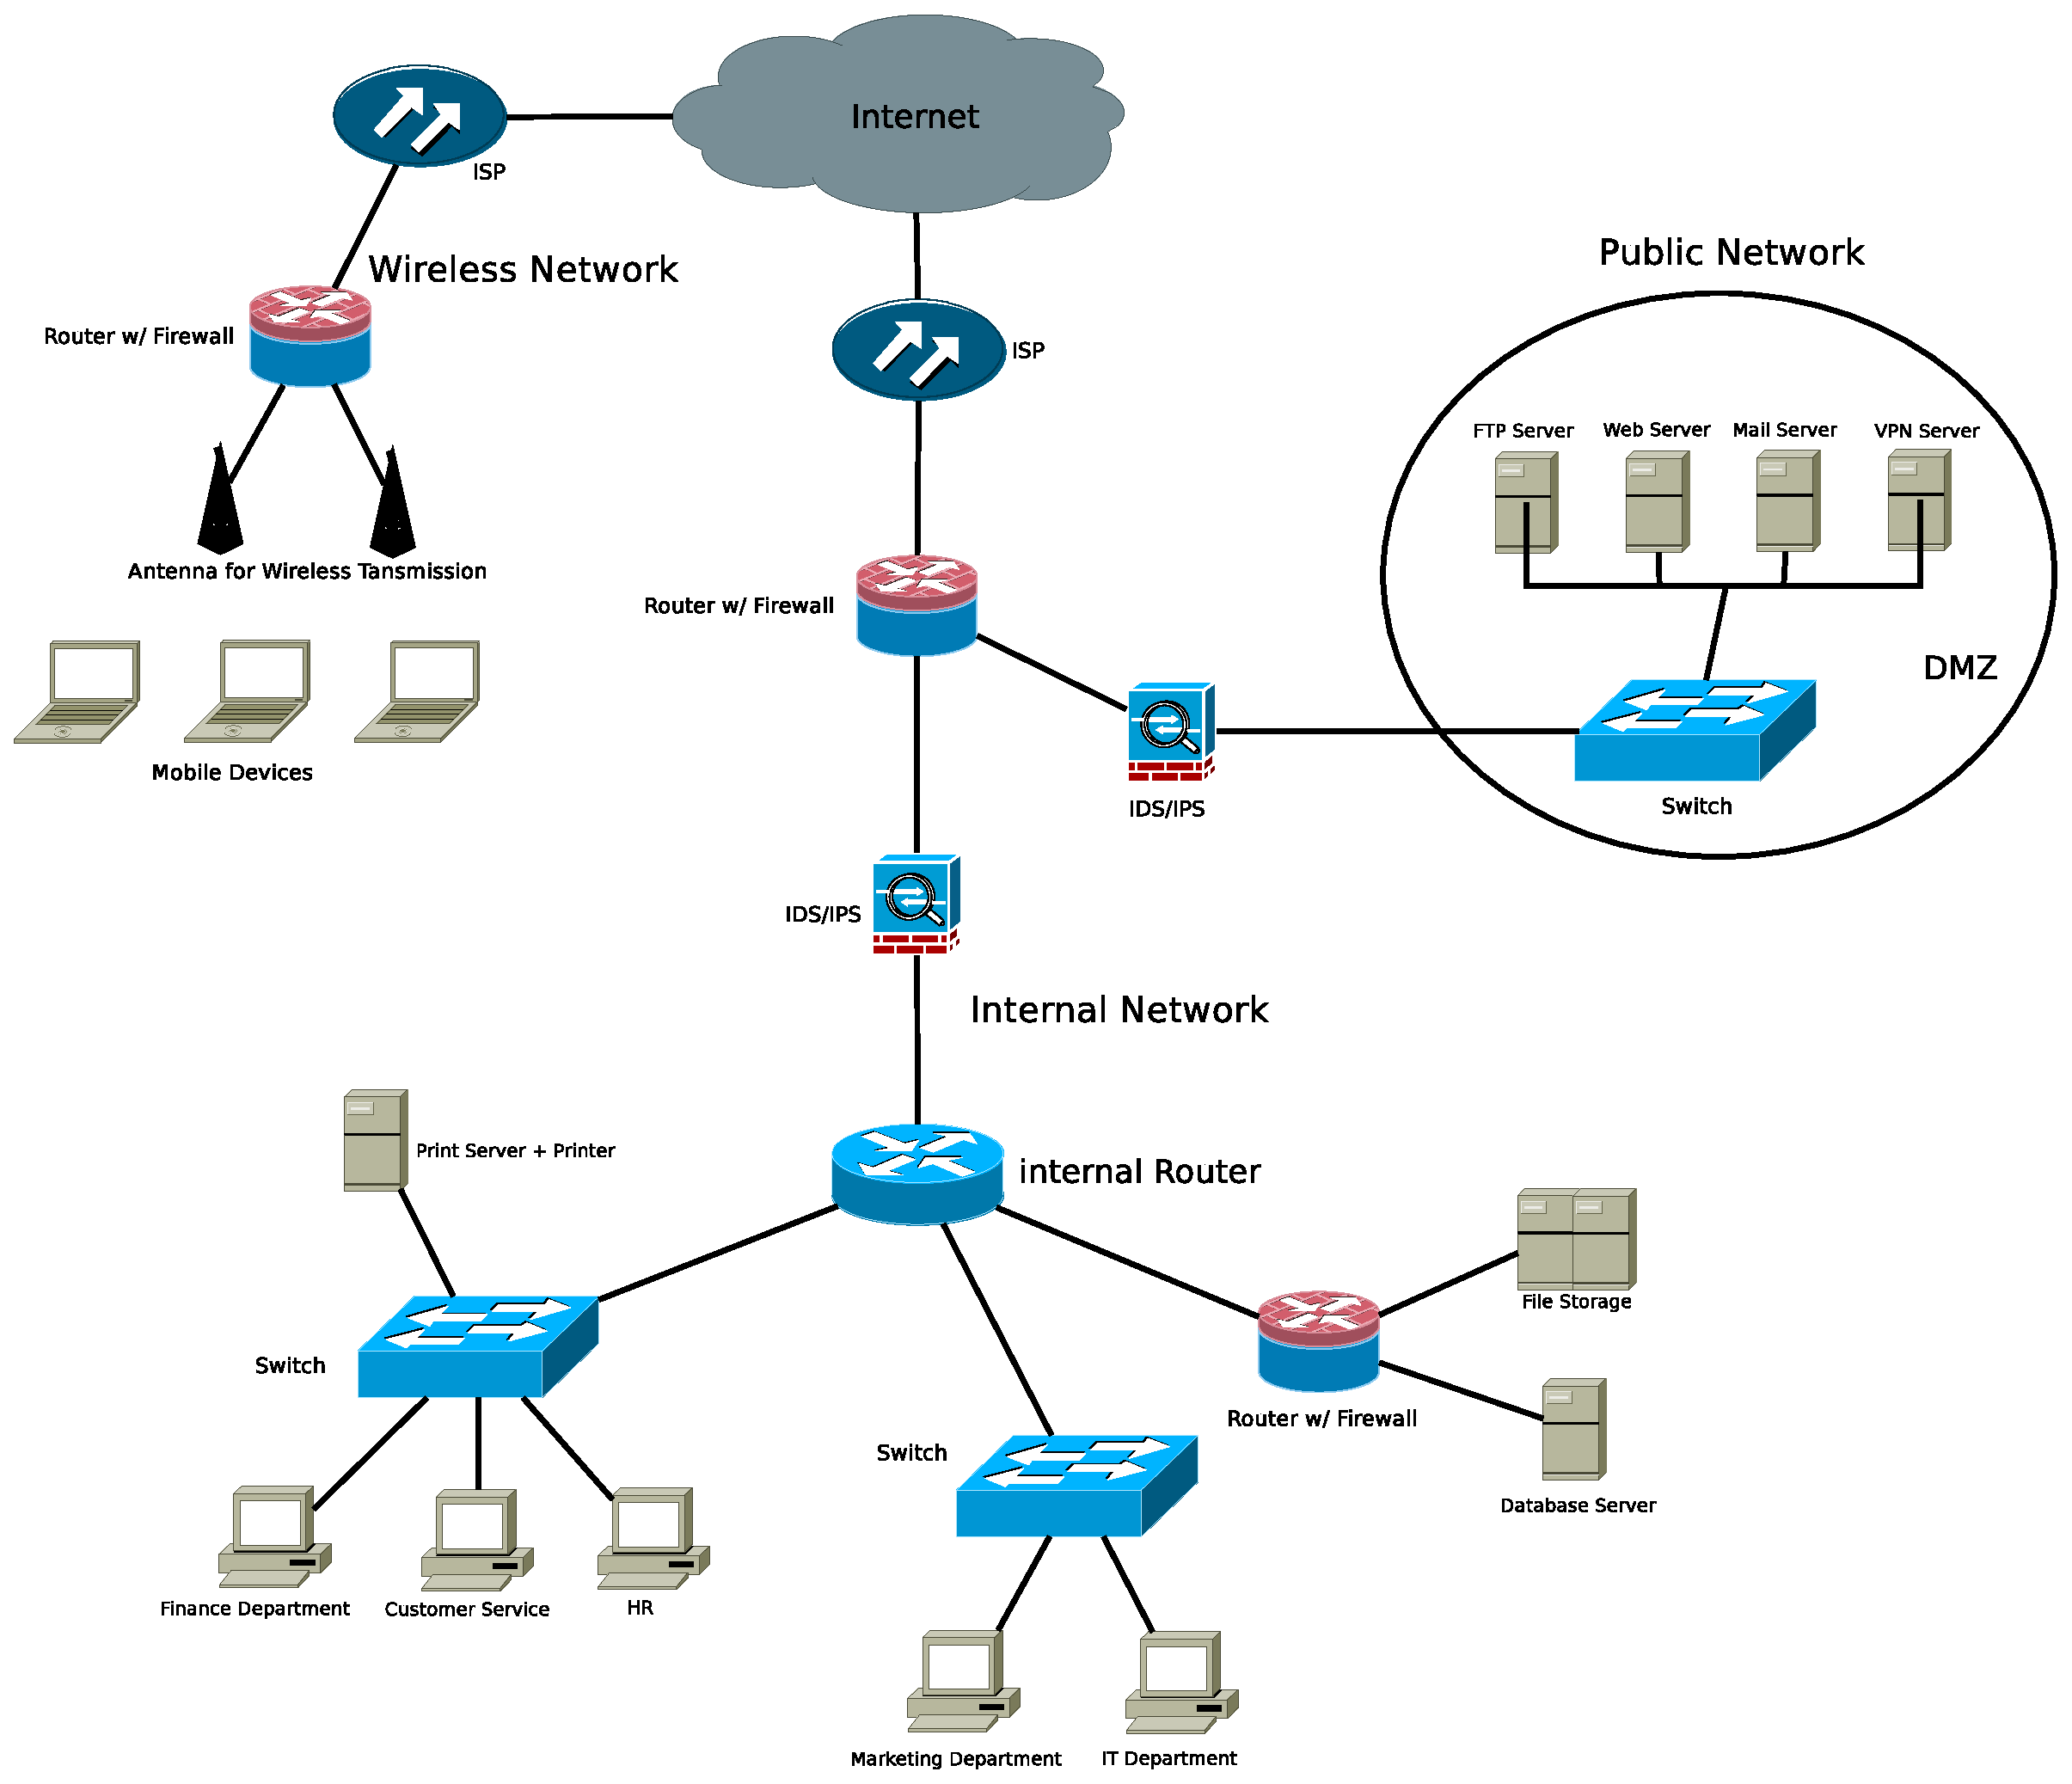
\includegraphics[scale=.3]{pictures/network_topology.eps}
	\caption{Network Topology}
	\label{fig:net_top}
\end{figure}
\subsection{Rules and Regulation}
As BYOD (bring your own device) is becoming more and more a security risk for companies, Smoking Games have strict policies for personal mobile devices. They are only allowed to use in the wireless area and (of course) outside the company network. Also, no information regarding the customers or business projects is allowed to keep or use on the devices. Flash drives provided by Smoking Games are encrypted and have an installed anti-spyware protable scanner to keep them free of malware. They are allowed to use inside the companies network, but not in the wireless area or outside of the building. The same applies for other mobile devices provided by Smoking Games.\\
All employees are required to properly secure their work equipment as a part of the employee contract they have signed with the company. In return the company promises to give adequate education on how to secure their equipment. This kind of security measures includes anti-virus,
secure communication, physical security, clear-desk policy and other relevant topics. Also, the security team has to make sure, that on every machine the latest security updates are installed.\\
Smoking Games have an incremental daily backup strategy and a complete back-up each Friday night. These back-ups are stored both on site and off site. The off site storage facility is a third party service provider, which complies with the same policies and legislative demands as Smoking Games.\\
\newpage
\section{Risk Identification}\label{RiskIdent}
A business like Smoking Games faces a wide variety of threats. Therefore it is necessary to consider every possible threat, what impact it might have on the business and how to control it. In the following we will focus on the realistic threads, while the unimportant threats are set aside, since the project's scope will otherwise overwhelm the organization's ability to plan.
\subsection{Threat Assessment}
Table \ref{tab:Threats1} represents threats to Smoking Games. Each threat is assessed on a scale of 1 to 10 (with 1 being low and 10 being high), regarding the level of danger or impact it has on the company, the cost to recover from, and the expenditure to prevent it.\\
\begin{table}[h]
	\centering
	\begin{tabular}{| l | l | l | l |}
		\hline
		\textbf{Threat Category} & \textbf{\parbox[t]{2cm}{Danger/\\Impact}} & \textbf{\parbox[t]{2cm}{Recovery\\Cost}} & \textbf{\parbox[t]{2cm}{Prevention\\Expenditure}}\\\hline
		Espionage or trespass & 10 & 8 & 7\\\hline
		Software attacks & 9 & 7 & 8\\\hline
		Human error or failure & 8 & 7 & -\\\hline
		Theft & 7 & 6 & 7\\\hline
		Compromises of intellectual property & 6 & 6 & 6\\\hline
		Sabotage or vandalism & 5 & 7 & 5\\\hline
		Technical software failures or errors & 4 & 6 & 5\\\hline
		Forces of nature & 8 & 8 & 7\\\hline
		\parbox[t]{5cm}{Deviations in quality of service from service providers} & 8 & 7 & 8\\\hline
		Technologial obsolescence & 4 & 6 & 6\\\hline
		Information extortion & 5 & 7 & 7\\\hline
	\end{tabular}
	\caption{Threats to Smoking Games}\label{tab:Threats1}
\end{table}


	\chapter{Business Impact Analysis}
The business impact analysis (BIA) is divided into five parts\cite{whitman1}. The first part deals with the analysis of the risk each threat poses to Smoking Games (see \ref{sec:IdentThreatsAttacks}). Following from this, the Business Unit Analysis (BUA) is being performed, which indicates how the business would suffer under the loss of a business function --ref--. In part three different scenarios of successful attacks are being discussed --ref--. From these attack scenarios, in part four, the costs of the best, worst and moste likely outcomes is being estimated --ref--. Finally, in part five the attack scenarios are being classified according to severity to determine which subordinate plan should deal with it --ref--.


\section{Identification of Threats and Attacks}\label{sec:IdentThreatsAttacks}
In this section the list of threats discovered in the risk identification process\ref{RiskIdent} is being converted into a prioritized list of attacks. For this a Weighted Business Risk Analysis (WBRA) is being performed: the threats are weighted with a 50-50 split between probability and consequence, though consequence is divided into damage cost (30\%) and repair cost (20\%). Each threat scenario is followed by a short discription, which gives an explanation about the weights that are given. It is arranged by the "Total" value (from high to low). Prioritization of each scenario is based upon which resources are most valuable to the company. Preservation of human lifes is always prioritized.\\
Table \ref{ref:tabWBRA} shows the results of the WBRA and is derived from table 2-2 \cite{whitman2}.\\
\begin{longtable}{| p{4.2cm} | p{1.8cm} | p{1.8cm} | p{1.8cm} | p{1.8cm} |}
		\caption{Weighted Business Risk Analysis}\label{ref:tabWBRA}\\
		%the following until endfirsthead goes on top of table on first page
		\hline \multicolumn{5}{|c|}{\textbf{Weighted Business Risk Analysis}}\\\hline
		\textbf{Threat} & \textbf{Probability (0.5)} & \textbf{Damage Cost (0.2)} & \textbf{Repair Cost (0.3)} & \textbf{Total (1.0)}\\\hline
		\endfirsthead
		%the following until endhead goes on top of table of every page except first page
		\textbf{Threat} & \textbf{Probability (0.5)} & \textbf{Damage Cost (0.2)} & \textbf{Repair Cost (0.3)} & \textbf{Total (1.0)}\\\hline
		\endhead
		%the following until endfoot goes at bottom of table except last page
		\multicolumn{5}{|c|}{\textit{continued on next page}}\\
		\endfoot
		%the following until endlastfoot goes at bottom of table on last page
		\endlastfoot
		Fire & 0.5 & 0.9 & 0.8 & 0.67\\\hline
		& \multicolumn{4}{|p{8cm}|}{\textit{The likelihood for a fire to occur is moderate because of the mostly warm weather; the damage cost is very high; the repair cost is high, because equipment or building parts need to be repaired.}}\\\hline
		Denial of service attack & 0.7 & 0.8 & 0.5 & 0.66\\\hline
		& \multicolumn{4}{|p{8cm}|}{\textit{Very likely to happen; would cause high damage, because customers/users won't have access to the servers.}}\\\hline
		Social engineering attack via e-mail & 0.8 & 0.6 & 0.4 & 0.64\\\hline
		& \multicolumn{4}{|p{8cm}|}{\textit{Very likely that some phishing e-mails will go through the spam-filter, but it would most likely cause minimal damage because of routines.}}\\\hline
		Information leakage & 0.5 & 0.8 & 0.8 & 0.63\\\hline
		& \multicolumn{4}{|p{8cm}|}{\textit{High damage and high risk. It also has a high cost because it is difficult to discover and most likely not fixable.}}\\\hline
		Strong winds & 0.7 & 0.5 & 0.6 & 0.63\\\hline
		& \multicolumn{4}{|p{8cm}|}{\textit{Likely to occur; the damage cost is moderate due to the fact Smoking Games does not have any assets exposed other than it may be temporary loss of third party services; the repair cost is also moderate since building damage needs to be repaired.}}\\\hline
		Vulcanic eruption & 0.5 & 0.6 & 0.8 & 0.61\\\hline
		& \multicolumn{4}{|p{8cm}|}{\textit{Vulcanic eruptions are very likely to happen due to the location; damage cost varies by severity; repair costs are high because systems/building need to be repaired/restored.}}\\\hline
		Loss of user equipmment & 0.6 & 0.3 & 0.7 & 0.57\\\hline
		& \multicolumn{4}{|p{8cm}|}{\textit{This is not uncommon since users might break or loose their equipment; the damage cost is moderate since it's only the equipment which is lost; the repair cost is also moderate to high since the euipment needs to be replaced.}}\\\hline
		Social engineering attack via phone & 0.5 & 0.6 & 0.6 & 0.55\\\hline
		& \multicolumn{4}{|p{8cm}|}{\textit{Likely to happen because the phone numbers are accessible through the website; the damage however would likely be small because of procedures against exactly this kind of incidents.}}\\\hline
		Destruction of project management system & 0.2 & 0.8 & 0.9 & 0.53\\\hline
		& \multicolumn{4}{|p{8cm}|}{\textit{The likelihood of someone destroying the project management system is low, though in the case of such an incident the damage cost is high; the repair cost is extreme due to the fact that it's necessary to repair, replace and restore the systems.}}\\\hline
		Unauthorized software installation & 0.6 & 0.5 & 0.4 & 0.52\\\hline
		& \multicolumn{4}{|p{8cm}|}{\textit{The probability for this act is low, but it will probably take time and resources to repair.}}\\\hline
		Destruction of finance system & 0.2 & 0.8 & 0.8 & 0.5\\\hline
		& \multicolumn{4}{|p{8cm}|}{\textit{Destruction of the finance system is very unlikely to happen; the damage is high due to loss of customer accounts and billing information; the cost of repairing this system is also significantly high due to the restoration and improving of the system.}}\\\hline
		Internet outage & 0.4 & 0.9 & 0.4 & 0.5\\\hline
		& \multicolumn{4}{|p{8cm}|}{\textit{Rather unlikely to happen; damage cost is very high, because customers/users can't access the servers;  repair cost is rather low, because in most cases the ISP needs to make sure Smoking Games is conencted to the Internet.}}\\\hline
		Loss of information & 0.5 & 0.4 & 0.5 & 0.48\\\hline
		& \multicolumn{4}{|p{8cm}|}{\textit{This is not uncommon since information is often transported by portable storage mediums; the damage cost is moderate since storage mediums are encrypted; repair cost is moderate since Smoking Games must initiate an investigation and then implement proper counter measures.}}\\\hline
		Lightning & 0.3 & 0.7 & 0.6 & 0.47\\\hline
		& \multicolumn{4}{|p{8cm}|}{\textit{The chances for this incident to occur is low due to in-place countermeasures; the damage cost is high because all the IT-system is connected to the infrastructure; repair cost is also high since the systems need to be repaired or restored.}}\\\hline
		Worm in the internal network & 0.3 & 0.7 & 0.6 & 0.47\\\hline
		& \multicolumn{4}{|p{8cm}|}{\textit{With strict access routines and well educated staff, the likelihood is small; the damage however could be very severe; it would take a moderate amount of time and resources to fix the network.}}\\\hline
		Water leakage & 0.3 & 0.7 & 0.6 & 0.47\\\hline
		& \multicolumn{4}{|p{8cm}|}{\textit{This happens rarely but can be costly and inconvenient when it does happen; both in external costs and resources wasted handling the incident.}}\\\hline
		Flood & 0.2 & 0.7 & 0.7 & 0.45\\\hline
		& \multicolumn{4}{|p{8cm}|}{\textit{The chance for a flood to occur is low; the damage cost to business for inability to properly function is moderate to high, as well es the repair costs.}}\\\hline
		Destruction of the buildings structure & 0.4 & 0.5 & 0.5 & 0.45\\\hline
		& \multicolumn{4}{|p{8cm}|}{\textit{This is a probable attack which may occur; the cost of the damage is moderate since it will result in lost work time and business functionality; the repair cost is also moderate due to the fact it results in higher rent, along with a split repair cost.}}\\\hline
		Unauthorized access to wireless network & 0.5 & 0.4 & 0.4 & 0.45\\\hline
		& \multicolumn{4}{|p{8cm}|}{\textit{A basic WPA2 encrypted network is unlikely to crack, but the network is very little used and would probably be detected early.}}\\\hline
		Unauthorized access to work laptop & 0.4 & 0.6 & 0.4 & 0.44\\\hline
		& \multicolumn{4}{|p{8cm}|}{\textit{All laptops are encrypted so the most likely attack vector is via malware; it does contain sensitive information and could be used to further attacks so the damage could be large.}}\\\hline
		Accidental deletion of data & 0.7 & 0.3 & 0.1 & 0.44\\\hline
		& \multicolumn{4}{|p{8cm}|}{\textit{Very likely to happen; usually this will not make a big difference to the organization mainly because of backups and subversion systems.}}\\\hline
		Theft of finances & 0.3 & 0.8 & 0.4 & 0.43\\\hline
		& \multicolumn{4}{|p{8cm}|}{\textit{This incident happens rarely, but may happen either by error or deliberately; the damage cost is high since it will result in loss of finances and possibly in large faults in the accounting and loss of employees; the repair cost is moderate since it will result in a complete revision of the accounting and lawsuits.}}\\\hline
		Destruction of access control system & 0.3 & 0.5 & 0.6 & 0.43\\\hline
		& \multicolumn{4}{|p{8cm}|}{\textit{The destruction of the access control system is not likely, but probable due to the fact of its exposed placements; the damage cost is moderate; the repair cost is somewhat higher due to the process of restoring and enhancing the system.}}\\\hline
		Sabotage of access control equipment & 0.5 & 0.4 & 0.3 & 0.42\\\hline
		& \multicolumn{4}{|p{8cm}|}{\textit{Sabotaging the access control system is likely to happen, since there are several people allowed to access it; the damage cost is moderate; the repair cost is low since it is an external service.}}\\\hline
		Sabotage of project and finance system & 0.3 & 0.3 & 0.7 & 0.42\\\hline
		& \multicolumn{4}{|p{8cm}|}{\textit{The chances of sabotaging either system is not very likely; the damage cost is low since the systems are properly secured and monitored; the repair cost is high due to the work needed to restore and improve the security, along with pursuing the incident.}}\\\hline
		Hard-disk on backup server crashes & 0.4 & 0.3 & 0.5 & 0.41\\\hline
		& \multicolumn{4}{|p{8cm}|}{\textit{The backup procedures are redundant which makes sure that there is more than one copy; most losses are based on time and resources spent; however, it is quiet likely to happen.}}\\\hline
		Unauthorized access to file server & 0.3 & 0.7 & 0.4 & 0.41\\\hline
		& \multicolumn{4}{|p{8cm}|}{\textit{The file server is placed securely on the internal network and to access it unauthorized is very difficult; it does contain sensitive information that could be severe if it falls into the wrong hands; backups make it easy to restore.}}\\\hline
		Functional bugs in 3rd party software & 0.6 & 0.2 & 0.2 & 0.40\\\hline
		& \multicolumn{4}{|p{8cm}|}{\textit{These kinds of bugs might have a slight impact on the business, but it will most likely be corrected fast and it will be barely noticeable.}}\\\hline
		Unauthorized access to database & 0.3 & 0.8 & 0.3 & 0.40\\\hline
		& \multicolumn{4}{|p{8cm}|}{\textit{The database is well secured on the internal network;  compromise could cause severe damage to reputation, but backups would help to restore it relatively easy.}}\\\hline
		Sabotage of physical documents & 0.4 & 0.7 & 0.3 & 0.38\\\hline
		& \multicolumn{4}{|p{8cm}|}{\textit{The chances of sabotaging physical documents is moderate since they are stored in a secured file cabinet; the damage cost is low; the repair cost is moderate since a complete check of the inventory has to be done.}}\\\hline
		Unauthorized access to VPN account & 0.3 & 0.4 & 0.5 & 0.38\\\hline
		& \multicolumn{4}{|p{8cm}|}{\textit{The biggest attack vector here is weak passwords for which there are strict routines against it; this is an intermediate attack which an attacker could use to further compromise assets.}}\\\hline	
		Web site defacement & 0.6 & 0.5 & 0.5 & 0.37\\\hline
		& \multicolumn{4}{|p{8cm}|}{\textit{Likely to happen; causes severe damage to reputation; the cost to repair would be moderate.}}\\\hline
		Accidental removal of critical equipment & 0.3 & 0.5 & 0.4 & 0.37\\\hline
		& \multicolumn{4}{|p{8cm}|}{\textit{The probability that this error will occur is low, but mistakes do happen; the impact of this will be moderate because critical equipment or information storage devices will be unaccounted for, but only temporary lost and not stolen.}}\\\hline
		Unauthorized physical access to restricted areas & 0.2 & 0.6 & 0.5 & 0.37\\\hline
		& \multicolumn{4}{|p{8cm}|}{\textit{These areas have enhanced security, which in return makes the cost of repairing and replacing the access control system higher.}}\\\hline
		Theft of information & 0.3 & 0.2 & 0.6 & 0.37\\\hline
		& \multicolumn{4}{|p{8cm}|}{\textit{Occurs rarely, but is not uncommon either; even though the damage cost is low since the information is encrypted and physical information is not to be of a sensitive nature; repair cost is moderate since Smoking Games must initiate an investigation and then implement proper counter measures.}}\\\hline
		Destruction of emergency systems & 0.3 & 0.5 & 0.4 & 0.37\\\hline
		& \multicolumn{4}{|p{8cm}|}{\textit{This is not likely, but still possible due to its natural placement and implementation; the damage cost is moderate, since it needs to be maintained; the repair cost is moderate, since it requires additional testing and repair work before its functional again.}}\\\hline
		Earthquake & 0.4 & 0.5 & 0.7 & 0.36\\\hline
		& \multicolumn{4}{|p{8cm}|}{\textit{Earthquakes are likle to occur because of the location; damage cost varies by severity of the earthquake; repair costs are high because it is necessary to replace and restore the systems/building.}}\\\hline
		Filing error & 0.5 & 0.1 & 0.3 & 0.36\\\hline
		& \multicolumn{4}{|p{8cm}|}{\textit{Happens from time to time, but no information is lost.}}\\\hline
		Hard-disk on laptop crashes & 0.4 & 0.3 & 0.3 & 0.35\\\hline
		& \multicolumn{4}{|p{8cm}|}{\textit{All employees are required to do backups regularly so most costs are replacing and configuring the new work environment.}}\\\hline
		Hard-disk on file server crashes & 0.4 & 0.3 & 0.3 & 0.35\\\hline
		& \multicolumn{4}{|p{8cm}|}{\textit{This would cause problems with the daily operation very fast, but good backup routines ensure that very little or no data will be lost.}}\\\hline
		Hard-disk on database server crashes & 0.4 & 0.3 & 0.3 & 0.35\\\hline
		& \multicolumn{4}{|p{8cm}|}{\textit{Good backup routines will make sure, that very little or no data is lost, but it still takes time recovering and cost to replace.}}\\\hline
		Hard-disk on web server crashes & 0.4 & 0.3 & 0.3 & 0.35\\\hline
		& \multicolumn{4}{|p{8cm}|}{\textit{A backup server is in place so there will be very little downtime; most costs are directed towards setting the environment to the previous standards.}}\\\hline
		Vendor stops supporting software & 0.2 & 0.5 & 0.5 & 0.35\\\hline
		& \multicolumn{4}{|p{8cm}|}{\textit{Vendors  rarely stop security updates to a product suddenly, if they do it might take considerable resources to update the systems.}}\\\hline
		Loss of access credentials & 0.6 & 0.1 & 0.4 & 0.35\\\hline
		& \multicolumn{4}{|p{8cm}|}{\textit{Loss of access credentials is not uncommon; the damage is not significant since employees is trained to report loss; the repair cost is moderate, since it is only a matter of disabling and issuing a new ID and PIN.}}\\\hline
		Unauthorized physical access to the premises & 0.3 & 0.4 & 0.4 & 0.35\\\hline
		& \multicolumn{4}{|p{8cm}|}{\textit{A proper physical security is implemented, the damage is covered by other threats; the damage cost and repair cost is for covering repair and replacement of the access control system.}}\\\hline
		Unauthorized physical access to Smoking Games's internal facilities & 0.1 & 0.6 & 0.5 & 0.32\\\hline
		& \multicolumn{4}{|p{8cm}|}{\textit{The areas within Smoking Games's office is also secured with enhanced security and the damage cost is covered by other threats.}}\\\hline
		Theft of access credentials & 0.3 & 0.3 & 0.3 & 0.30\\\hline
		& \multicolumn{4}{|p{8cm}|}{\textit{Happens rarely; the damage is not severe since employees are trained to report this type of incident; the repair cost is low since it only involves disabling and issuing a new ID-card with a new PIN.}}\\\hline
		Theft of user equipment & 0.2 & 0.3 & 0.4 & 0.28\\\hline
		& \multicolumn{4}{|p{8cm}|}{\textit{Happens rarely; the damage cost is moderate since it contains information and access to the business secured network, though the entire system is encrypted and will wipe itself in case of theft; the repair cost is moderate since it's necessary to replace the equipment and implement mitigating controls for the incident.}}\\\hline
		Power outage & 0.4 & 0.2 & 0.1 & 0.27\\\hline
		& \multicolumn{4}{|p{8cm}|}{\textit{This happens rarely and is usually very short when it does happen; a backup-power-generator will operate in case of emergency.}}\\\hline
\end{longtable}


%information leakage
%social engineering attack via email
%destruction of project management system
%flood, lightning, fire, earthquake, tsunami
%unauthorized software installation
%loss of information
%worm in the internal network
%water leakage
%destruction of the buildings structure
%unauthorized access to wireless network
%destruction of finance system
%loss of user equipmment
%unauthorized access to work laptop
%accidental deletion of data
%sabotage of access control eqipment
%sabotage of project and finance system
%hard disk on backup server crashes
%unauthorized access to file server
%functional bugs in 3rd party software
%theft of finances
%sabotage of physical documents
%unauthorized access to database
%unauthorized access to VPN account
%web site defacement
%accidental removal of critical equipment
%unauthorized physical access to restricted areas
%unauthorized physical access to Smoking Games's internal facilities
%filing error
%social engineering attack via phone
%hard disk on laptop crashes
%hard disk on file server crashes
%hard disk on database server crashes
%hard disk on web server crashes
%vendor stops supporting software
%loss of access redentials
%unauthorized physical access to the premises
%theft of information
%decial of service against assets
%destruction of access control system
%destruction of emergency systems
%theft of user equipment
%power outage
%theft of access credentials
%string winds
%internet outage
%power burnout


%\subsection{Business Processes and Recovery Criticality}
%Smoking Games's can roughly be divided into 4 business areas: financial system, business intelligence (e.g. project managers), sales and marketing, and game/software development. In order to keep the company in business, it is crucial to determine the business processes of each business area and evaluate them based on costs of failure. This includes the outage of a process, the delay, and the longest time a process could be left without being performed.
%\begin{table}[h]
%	\centering
%	\begin{tabular}{| l | c | c | c | c | c |}
%		\hline
%		\textbf{\parbox[t]{2cm}{Business\\Function}} & \textbf{\parbox[t]{2cm}{Impact on\\Profitability\\(40\%)}} & \textbf{\parbox[t]{2cm}{Contribution to\\Strategic\\Objectives\\(30\%)}} & \textbf{\parbox[t]{2cm}{Impact on\\Internal\\Operations\\(20\%)}} & \textbf{\parbox[t]{2cm}{Impact on\\Public Image\\(10\%)}} & \textbf{\parbox[t]{2cm}{Total\\Weights\\(100\%)}}\\\hline
%		Providing Internet services
%		
%	\end{tabular}
%	\caption{Weighted Business Risk Analysis}\label{ref:tabWBRA}
%\end{table}



%\input{Chapters/Business_impact_analysis/}
%\input{Chapters/Business_impact_analysis/}
%\input{Chapters/Business_impact_analysis/}
	%\input{Chapters/}
	%\input{Chapters/}
	%\input{Chapters/}
	%\input{Chapters/}
	%\input{Chapters/}

	%% Bibliography
	\bibliographystyle{unsrt}
	\bibliography{main}
	\begin{thebibliography}{99}
		\bibitem{whitman1}
			Michael E. Whitman and Herbert J. Mattford.
			\emph{Principles of Incident Response and Disaster Recovery}.
			pages 55–69.
			Course Technology, 2007.
			
		\bibitem{whitman2}
			Michael E. Whitman and Herbert J. Mattford.
			\emph{Principles of Incident Response and Disaster Recovery}.
			chapter 2, 	pages 60–61.
			Course Technology, 2007.
			Table 2-2.
	\end{thebibliography}

	%% APPENDICES
	\appendix %after this line all chapters will have leters instead of numbers
%	
\chapter{Basic information}
Table \ref{tab:emergency_call}, \ref{tab:emergency_loc} and \ref{tab:emergency_out} are based on templates from the book Principles of incident response and disaster recovery \quote{} which was collected from Texas State library\quote{}

\begin{longtable}{| p{4cm}  p{4cm}  p{4cm}|}
	\label{tab:emergency_call}
	\caption{ An example over how an Emergency call sheet might look like, some sample emergencies are included.}
	\hline \multicolumn{2}{| c |}{\textbf{Emergency call sheet}}\\\hline
	\endfirsthead
	
	\hline \multicolumn{2}{| c |}{\textbf{Emergency call sheet}}\\\hline
	\endhead
	
	\multicolumn{2}{|r|}{\textit{continued on next page}}\\\hline
	\endfoot
	
	\endlastfoot
	
	\textbf{Service:} & \textbf{Contact person:} & \textbf{Number:}\\\hline
	Ambulance & Aspirino Gonzalez Madro\~no & 141 592 653 \\
	Police & Officer Torrente & 589 793 238 \\
	Fire department & Helena los del Rio & 462 643 383 \\
	Electrician & Manolo el del Bombo & 279 502 884 \\
	Plumber & Alfonzo Torrente & 197 169 399 \\\hline	
\end{longtable}

\begin{longtable}{| p{4cm}  p{4cm}  p{4cm}|}
	\label{tab:emergency_loc}
	\caption{ An example of how to enumerate all emergency equipment, should be placed on map.}
	\hline \multicolumn{2}{| c |}{\textbf{Location of emergency system}}\\\hline
	\endfirsthead
	
	\hline \multicolumn{2}{| c |}{\textbf{Location of emergency system}}\\\hline
	\endhead
	
	\multicolumn{2}{|r|}{\textit{continued on next page}}\\\hline
	\endfoot
	
	\endlastfoot
	
	\textbf{Emergency:} & \textbf{Placement:} & \\\hline
	Fire extinguisher & At the meeting room & \\
	Electricity & Basement & \\\hline	
\end{longtable}

\begin{longtable}{| p{4cm}  p{4cm}  p{4cm}|}
	\label{tab:emergency_out}
	\caption{ An example of how to enumerate all equipment not in company care, and how to reach a contact employee.}
	\hline \multicolumn{2}{| c |}{\textbf{Equipment outside the company}}\\\hline
	\endfirsthead
	
	\hline \multicolumn{2}{| c |}{\textbf{Equipment outside the company}}\\\hline
	\endhead
	
	\multicolumn{2}{|r|}{\textit{continued on next page}}\\\hline
	\endfoot
	
	\endlastfoot
	
	\textbf{Item:} & \textbf{Contact/company:} & \textbf{Number:}\\\hline
	Backup web server & jaja.com & 375105820\\
	Security & Securitas direct & 974944592\\
	Water supply & Elcanal & 307816406\\\hline	
\end{longtable}

The numbers in table \ref{tab:salvage_prio} are based on the following criteria. The rating is inspired by the book Principles of incident response and disaster recovery\quote{}.
\begin{enum}
\item Salvage at all costs.
\item Salvage if time allows it.
\item Dispose of as part of general cleanup.
\end{enum}

\begin{longtable}{| p{4cm}  p{4cm}  p{4cm}|}
	\label{tab:salvage_prio}
	\caption{ List of all assets in priority human lives are not in the list, but always have top priority. This list shall be followed when several assets are at risk from one or several incidents at the same time.}
	\hline \multicolumn{2}{| c |}{\textbf{Salvage priority list}}\\\hline
	\endfirsthead
	
	\hline \multicolumn{2}{| c |}{\textbf{Salvage priority list}}\\\hline
	\endhead
	
	\multicolumn{2}{|r|}{\textit{continued on next page}}\\\hline
	\endfoot
	
	\endlastfoot
	
	\textbf{Item:} & \textbf{Location:} & \textbf{Priority:}\\\hline
	Backups & Basement & 1\\
	Personal Computers & At personal desk & 2\\
	Database servers & 2nd floor & 2\\
	File servers & 2nd floor & 2 \\
	Other servers & 3rd floor & 2 \\
	Non storage equipment over 1000000ptas & All the building & 2 \\
	Non storage equipment under 1000000ptas & All the building & 3 \\\hline	
\end{longtable}
\chapter{Inter-company Contact Info}



\begin{longtable}{| p{4cm} | p{2cm}  p{2cm} | p{4cm}|}
	\label{tab:contact_info}
	\caption{ Call sheet for leader positions that are responsible for handling an incident.}
	\hline \multicolumn{2}{| c |}{\textbf{Company Call sheet}}\\\hline
	\textbf{Position:} & \textbf{1.Number:} & \textbf{2.Number:} & \textbf{email:} \\\hline
	\endfirsthead
	
	\hline \multicolumn{2}{| c |}{\textbf{Company Call sheet}...continued}\\\hline
	\textbf{Position:} & \textbf{1.Number:} & \textbf{2.Number:} & \textbf{email:} \\\hline
	\endhead
	
	\multicolumn{2}{|r|}{\textit{continued on next page}}\\\hline
	\endfoot
	
	\endlastfoot
	
	Chief executive officer & 286 208 998 & 628 034 825 & ceo@smoke.com \\
	Chief marketing officer & 342 117 067 & 982 148 086 & cmo@smoke.com \\
	Chief Financial Officer & 513 282 306 & 647 093 844 & cfo@smoke.com \\
	Chief Technical Officer & 609 550 582 & 231 725 359 & cto@smoke.com \\
	IT manager & 408 128 481 & 117 450 284 & it@smoke.com \\\hline
\end{longable}
	%include file for all appendices

\end{document}

